\documentclass[a4paper]{article}

\usepackage{fullpage} % Package to use full page
\usepackage{parskip} % Package to tweak paragraph skipping
\usepackage{tikz} % Package for drawing
\usepackage{amsmath}
\usepackage{amssymb}
\usepackage{hyperref}
\usepackage{multirow}
\usepackage{booktabs}


\title{Programming Assignment 2 : Strassen's Algorithm}
\author{HUIDS: 90978217 AND 10978211}
\date{03/24/2017}

\begin{document}

\maketitle

\section{Overview}
In this programming assignment, we implement an optimized version of Strassen's algorithm to multiply two $n$ by $n$ matrices. Because Strassen's is slower than conventional matrix multiplication for sufficiently small matrices, our algorithm uses Strassen's algorithm for matrices down to a certain threshold size $n_0$, at which point which we utilize standard matrix multiplication. We determine $n_0$ both analytically and experimentally. The results from our studies are presented in this report.

Our code may be run by executing the following commands in the terminal:
\begin{verbatim}
$ make
$ ./strassen <verbosity> <dimension> <inputfile>
\end{verbatim}
where \texttt{verbosity} specifies the verbosity of the output (-1 for no output, 0 for the minimal output specified in the specs, 1 for more detailed output including matrix statistics).

\section{Method}
\subsection{Algorithm}
In this paper, we consider only matrix multiplication on square, integer valued matrices. We implement a modification of Strassen's algorithm, switching to using conventional matrix multiplication for matrices of size $m \leq n_0$. We determine the best crossover point both analytically and empirically in section 3.

Noting that Strassen's breaks the multiplication of $n$ by $n$ matrices into several multiplications of $n/2$ matrices, the first consideration in this implementation is modifying the formulation to handle matrices with sizes that are \textit{not} a power of 2. One solution is to pre-pad the input matrices, $A$ and $B$ to the smallest power of 2 such that $2^k \geq n$, filling the padded areas with 0's, and removing this padding after the product is computed to obtain the final output matrix. (The padding is applied to the bottom and right columns of the matrix). This approach is simple and relatively fast, allowing us to simply compute the product using naive Strassen's after the inital pad. We improve the efficiency of this static padding approach by noting that switching to conventional matrix multiplication beyond a crossover point $n_0$ means that we need only pad our matrices up the smallest size $m$ such that $m = 2^k n_0 \geq n$. We implement this optimized static padding in our solution.

When considering how to pad our matrices to obtain the appropriate dimensions, we also considered dynamic padding. Dynamic padding works by adding an extra row and column of padding only if the matrices being multiplied have an odd dimension, and then removing these extra 0s after the two matrices are multiplied; instead of pre-padding the entire input matrices, we pad ``on the fly'', only adding a row or column as necessary. This method mitigates the costs of multiplying unnecessarily large matrices (a possible concern in static padding), and is a direction for future work. We do not implement this solution here due to the added complexity of inferring information about submatrices' padding: For this approach, physically storing the padding is difficult, so any implementation would instead simply infer that the last row or column is populated with 0's if the dimension is not even and use this in calculations.

Once we have correctly-sized starting matrices, we recursively call Strassen's algorithm on inputs $A$ and $B$ until the submatrix sizes are less than or equal to the crossover point, $n_0$, at which point we switch to standard matrix multiplication. On inputs of size $k$, Strassen's requires us at each recursive level to calculate seven temporary matrix subproducts of size $k/2$ and add different combinations of these subproducts up to achieve our final output matrix $C$. 

To optimize for space and avoid storing each of these subproducts in memory, we store most of the intermediate subproducts in the output matrix $C$ at each level, storing the subproducts in such an order that we only require two temporary storage matrices $T_1, T_2$ of size $k/2$ each. [Table 1] To optimize for time efficiency, we chose to implement Winograd's variant of Strassen's algorithm. Winograd's variant conducts computations in a way that requires only 15 submatrix additions at each recursive level, as opposed to 18 additions for the original Strassen formulation [Li, Junjie, Sanjay Ranka, and Sartaj Sahni. "Strassen's matrix multiplication on GPUs." \textit{Parallel and Distributed Systems (ICPADS), 2011 IEEE 17th International Conference on.} IEEE, 2011.]

\begin{figure}[h]
	\caption{Order of computations for Douglas's implementation of Winograd's variant. Table taken from (Li et. al., 2011).}
	\centering
		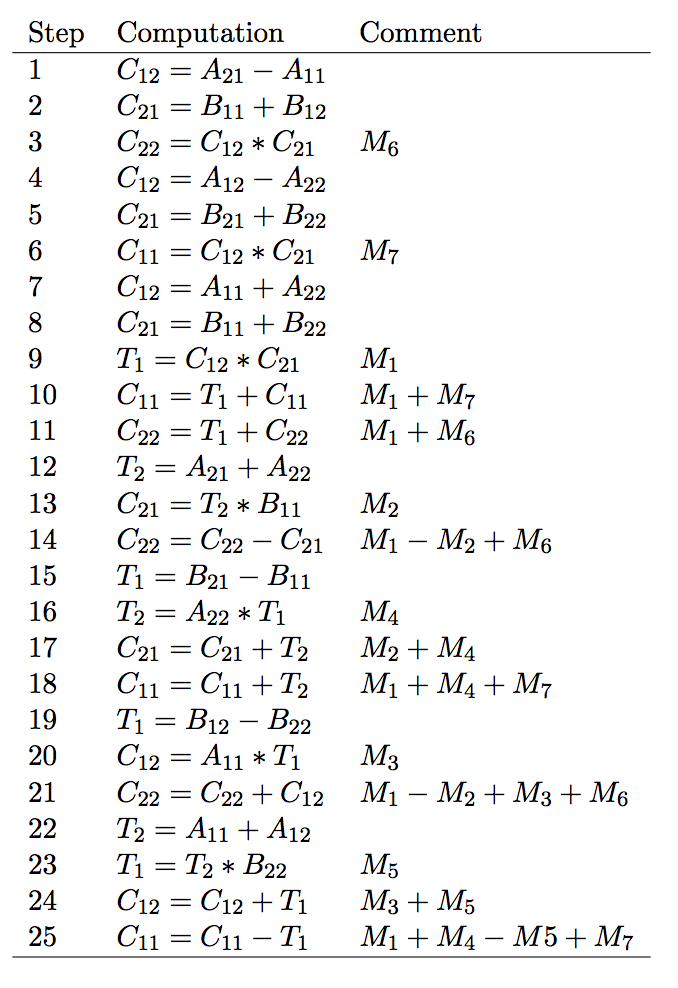
\includegraphics[width=3in]{computations.png}
\end{figure}

Once Strassen's algorithm decomposes into size $m\leq n_0$ matrices, we implement an optimized version of standard matrix multiplication, which simply swaps the order of the three loops necessary to compute the matrix product, from $ijk$ to $ikj$. Noting that C arrays are stored in row-major order, we can see that accessing elements in 1 row repeatedly leads to a much higher cache hit rate than accessing elements in 1 column repeatedly, allowing us to take advantage of hardware prefetching. Thus, we can modify the original algorithm, which computes \texttt{C[i, j] += A[i, k] B[k, j]} by looping through the indices in the order $ijk$, to instead loop in the order $ikj$.

\textbf{Runtime.} As discussed in class, the conventional matrix multiplication algorithm runs in $\Theta(n^3)$, while Strassen's original algorithm runs in time $\Theta(n^{log_27})$ for matrices with sizes of $2^k$.

To obtain a more accurate runtime for our generalized algorithm, note that the crossover + Winograd's variant of Strassen's algorithm has the following runtime recurrence relation for square matrices of size $n$:
\[ 
T(n) = 
\begin{cases} 
R(n) & n\leq n_0 \\
7T(n/2) + 15(n/2)^2 & o.w.
\end{cases}
\]
where $T(n)$ is the runtime for our algorithm, and $R(n) = n^2(n + n-1)$ is the runtime for the conventional matrix multiplication algorithm. For initial matrices of size $m$, we obtain statically padded matrices of size $n = \min(2^kn_0\mid2^kn_0\geq m)$. Expanding the recurrence for $T(n)$, we have the following closed form runtime for our algorithm:
\begin{align*}
T(n) &= 7^k(2n_0^3 - n_0^2) + 15\sum_{i=1}^k 7^{i-1}\left(\frac{n}{2^i}\right)^2 \\
&= 7^k(2n_0^3 - n_0^2) + 5 n_0^2(7^k - 4^k)
\end{align*}
for all initial matrices of size $2^{k-1}n_0 < m \leq 2^k n_0$; the runtime is a stepwise function, stepping at each padded matrix size.

\textbf{Space. } The space used by the algorithm can be found by noting that each call uses $2(n/2)^2 + n^2 = 3n^2/2$ space for matrices, and summing across one path in the recursion tree.
\begin{align*}
S(n) &= n_0^2 + \frac{3n_0^2}{2}\sum_{i=1}^k 4^i \\
&= n_0^2(2^{2k+1} - 1)
\end{align*}



\subsection{Implementation}
Our implementation of the algorithm can be found in two files: (1) \texttt{strassen.c}, which contains the functions for performing conventional and optimized matrix multiplication, command line parsing, and empirical threshold optimization, and (2) \texttt{strassen.h}, which contains various matrix helper functions including accessing matrix elements, adding/subtracting matrices, and padding. We choose to store our matrices in a continuous block of heap memory in row-major order, and access matrix elements by stepping by the matrix dimension: \texttt{m[i, j] = M[i * sz + j]}. 

To avoid repeated copying of submatrices during Strassen's, we instead simply pass the pointer to the top left corner of the submatrix to the recursive multiplication function, along with the submatrix size and the ``stride''. (The stride is used to find the $i,j$th element in the submatrix-- see code for more details.) Together, these arguments allow us to retrieve all elements in the submatrix without copying each submatrix to a newly allocated chunk of memory. Thus, our implementation only uses 2 temporary scratch matrices and 1 final output matrix at each call in the recursion, for a total of $n^2/2 + n^2 = 3n^2/2$ space at a call.

\section{Results and Discussion}

\subsection{Analytically determining threshold}
We analytically determine a crude approximation to the cross-over point $n_0$ at which the standard matrix multiplication algorithm runs more quickly than Strassen's algorithm.

First, we note that the standard matrix multiplication algorithm requires $n$ multiplications and $n-1$ additions for each of the $n^2$ entries in the output. As before, we have a runtime of
$$R(n) = n^2(n + (n-1)) = 2n^3 - n^2$$

The Winograd variant of Strassen's matrix multiplication algorithm decomposes each input matrix of size $n$ into seven multiplications of submatrices of size $n/2$, along with 15 additions of matrices of size $n/2$ [Table 1]. For simplicity, we consider the dynamically padded generalization of Strassen's for odd-sized matrices, which operates on submatrices of size $\lceil n/2\rceil$ after padding by one row and column if necessary. Combining, we can describe the runtime of our algorithm via the following recurrence equation: 
$$T(n) = 7T(\lceil n/2\rceil) + 15(\lceil n/2\rceil)^2$$
Noting that our optimized version of Winograd uses conventional matrix multiplication once the recursive calls reach inputs of size $\leq n_0$, we can obtain a crossover point by finding the $n_0$ such that the standard approach has runtime less than or equal to one iteration of Strassen's, followed by the use of the standard algorithm. Thus, because our base case for the recursive algorithm is $T(n_0) = R(n_0)$, to obtain $n_0$ we can solve the following inequality:
\begin{align*}
R(n_0) &\leq 7R(\lceil n_0/2\rceil) + 15(\lceil n_0/2\rceil)^2 \\
\iff 2n_0^3-n_0^2 &\leq 2(\lceil n_0/2\rceil)^3 - (\lceil n_0/2\rceil)^2 + 15(\lceil n_0/2\rceil)^2
\end{align*}
Solving for $n_0$ gives us an analytical solution of $n_0 \leq 12$.


\subsection{Experimentally determining threshold}

We experimentally determine the cross-over point $n_0$ at which the standard matrix multiplication algorithm runs more quickly than Strassen's algorithm.

We tested our algorithm for matrices of various sizes up to $n=1024$. For each $n$ we tested, we iterated over all possible threshold values to determine the threshold value $n_0$ that optimized the runtime of our algorithm (averaged across multiple trials). The results of our experiment are plotted below: \\

\begin{centering}
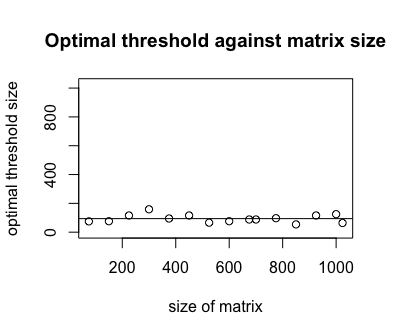
\includegraphics[width=3in]{threshplot} \\
\end{centering}

Examining these results, we did not notice a significant correlation between $n_0$ and $n$, suggesting a constant $n_0$ independent of $n$. This is not surprising, since the crossover point should be a fixed value based on the details of the two algorithms themselves, rather than the size of the input matrices (see section 3.1 for more details).

Taking the average $n_0$ across all $n$, we determined the experimentally optimal $n_0$ to be roughly \textbf{94}. Unsurprisingly, this value is of the same magnitude as our crude analytical estimate of \textbf{12}. (Note: the variation can likely be attributed to computer-specific considerations, as well as different caching considerations arising from how we stored our submatrices and accessed our elements via stepping.)

Notably, our code runs quite quickly, taking less than 0.05 seconds on average to multiply two matrices of size $n = 525$ (for the optimal $n_0$) and less than 0.5 seconds on average for size $n = 1024$. We plot the runtimes (based on the optimal $n_0$) for various $n$ below: \\

\begin{centering}
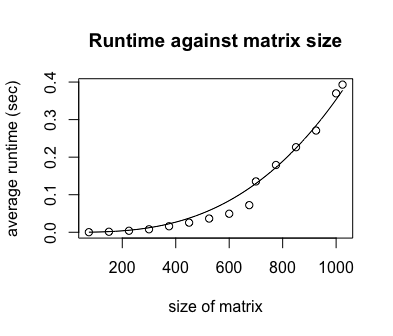
\includegraphics[width=3in]{timeplot} \\
\end{centering}

After running nonlinear least-squares regression in R, we note that the best fit line $$t(n) = 1.3e-09 \times n^{log_27}$$
is a good fit for the data. This is unsurprising given our prior analysis of Strassen's as running in $\Theta(n^{log_27})$.


\end{document}